\documentclass[12pt, a4paper]{article}
\addtolength{\oddsidemargin}{-.875in}
\addtolength{\evensidemargin}{-.875in}
\addtolength{\textwidth}{1.75in}
\addtolength{\topmargin}{-.875in}
\addtolength{\textheight}{1.75in}

\usepackage{indentfirst}
\usepackage{graphicx}
\usepackage{amsmath}


\begin{document}
\noindent
Nicholas Garrett\\ \\
Professor Fouda\\ \\
CS 4461\\ \\
1/28/2022\\ \\


\begin{center}
	\centering{	Homework 1\\ }
\end{center}

\noindent
Chapter 4\\

4.1.

	I would assume that because the script says ``System will switch when the current process is FINISHED'', that the CPU will have a 100\% time use.  \\
	\begin{center}
	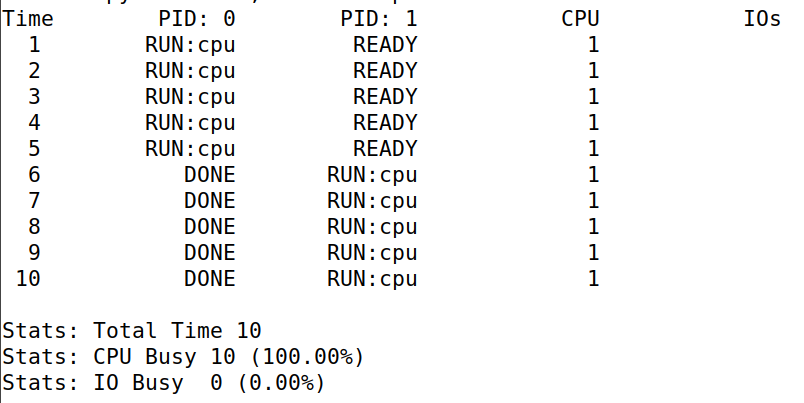
\includegraphics[width=6cm]{hw1_4_1.png}\\
	\end{center}
	
	From the output of the code with -c and -p flags, it appears I was correct in my answer.\\ \\ \\
	
4.2.

	I would assume that since the flags specify a single process to run with four instructions and a single I/O wait operation, that it would take four ticks to complete the first process and something more than that to finish both processes.\\
	\begin{center}
	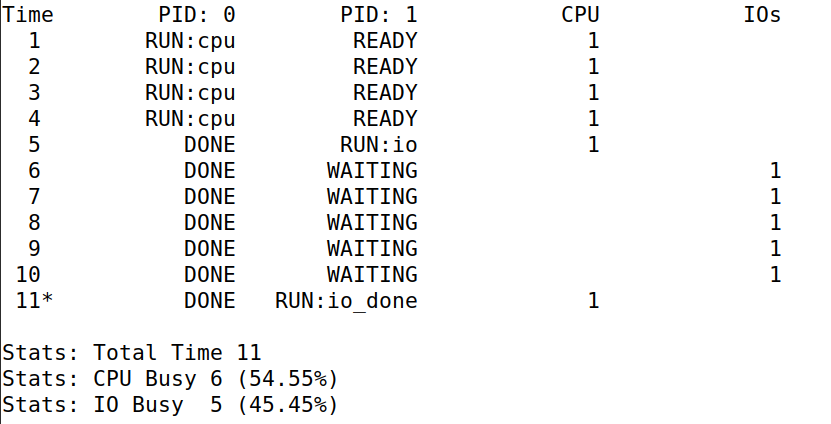
\includegraphics[width=6cm]{hw1_4_2.png}\\
	\end{center}
	
	From the code output, it appears that there are six busy CPU ticks. I had not considered that the I/O complete would itself take a tick. \\ \\ \\
	
4.3

	I would assume that because the CPU will set the process checking IO to wait, the four operations will run while the I/O waits. Therefore, I think that this configuration might be able to run in as little as 6 processes. \\
	\begin{center}
	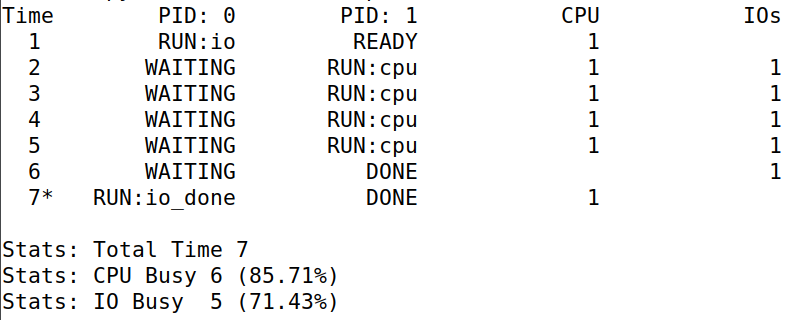
\includegraphics[width=6cm]{hw1_4_3.png}\\
	\end{center}
	
	From the output, it looks like this assessment was correct, though a single tick occured where the CPU was no longer running the four operations though was still waiting on the I/O operation. \\ \\ \\

4.4

	From the explanation of the flag set, the logical outcome of running the script with its I/O process being followed by four operations is that the number of ticks required is whatever number is required to operate the I/O followed by four process ticks.\\
	
	\begin{center}
	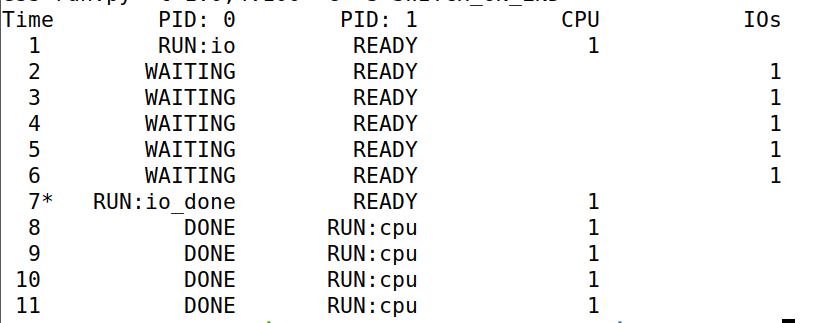
\includegraphics[width=6cm]{hw1_4_4.png}\\
	\end{center}
	
	From the code's output, it looks like this assessment is correct. \\ \\ \\
	

4.5

	Based on the description of how the SWITCH\_ON\_IO flag operates, I would assume that this call will lead to the four processes starting as soon as the WAIT command occurs on the I/O-dependant process.
	
	\begin{center}
	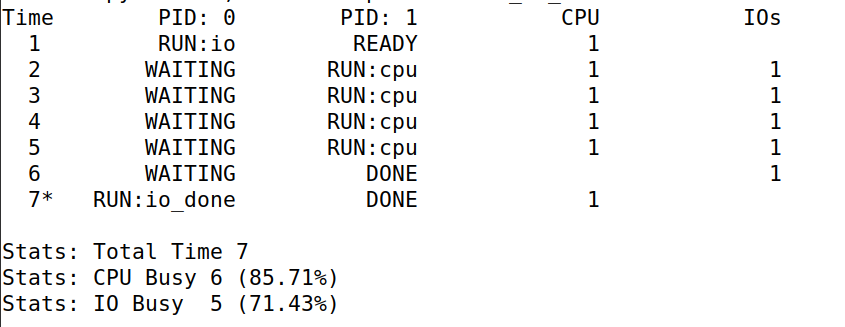
\includegraphics[width=6cm]{hw1_4_5.png}\\
	\end{center}

	From the console output, it looks like this assessment was correct. \\ \\ \\
	
4.6
	From the description of how the flags operate, I think that the first I/O process will start, then WAIT for the I/O response. During this time, the five processes following it will run. And if it is still not done, then the five processes following them will run, etc. After those processes, I expect the other two I/O dependent processes will run. 
	
	
	\begin{center}
	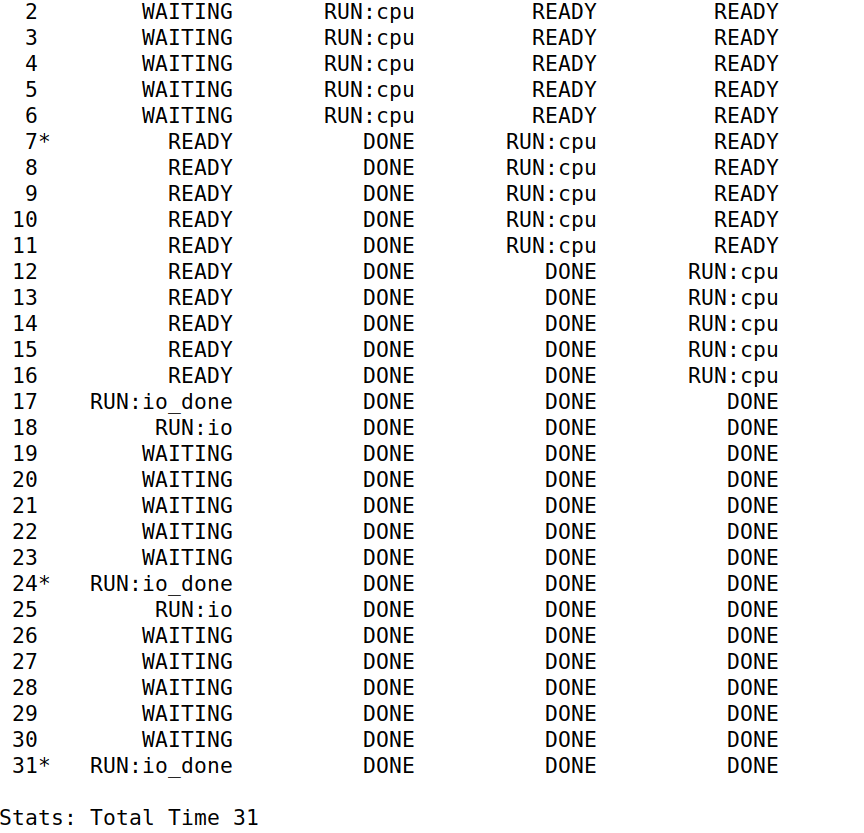
\includegraphics[width=6cm]{hw1_4_6.png}\\
	\end{center}

	From the output generated, it looks like my presumption was wrong. It looks like the I/O process started then waited for the I/O return. I had assumed that only one or two of the 5-operation processes would execute before the next I/O process. Though, it looks like they all ran, even after the I/O process was ready. 
	
	I say that this is inefficient because it leaves I/O processes to execute afterwards, which leave unused CPU time where it simply waits for I/O return. \\ \\ \\

4.7
	
	With the new execution flags, it sounds like the I/O process will run then wait. During this time, the five processes following it will run. Then the I/O process will continue to execute, which will run its second I/O call and wait, during which time the next five processes will run, and the same thing will happen again.
	
	\begin{center}
	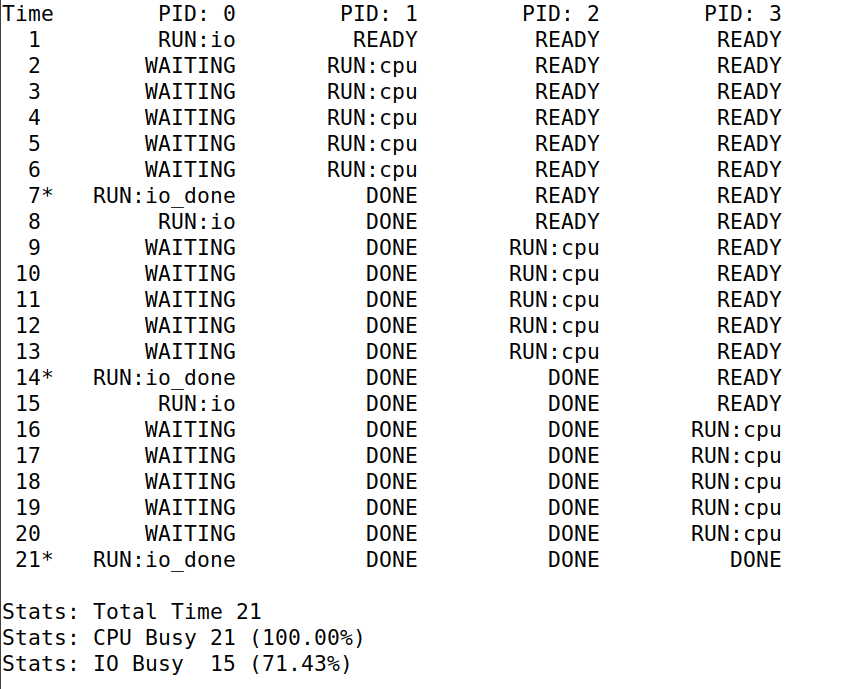
\includegraphics[width=6cm]{hw1_4_7.png}\\
	\end{center}
	
	From the output, it looks like this assessment is correct. The executed code runs much more efficiently this time, keeping the CPU busy at 100\%. Running the processes that had just made an I/O cal again helps to improve efficiency if they call multiple I/O returns.l \\ \\ \\

4.8

	From what I have learned while doing this assignment, I think that the first process will run, then wait on its I/O. During this time, the second process will run and wait on its I/O. The first process will run next as its I/O call should finish first and will finish, followed by the second process.
	
	************uncompleted**************	 \\ \\ \\
	



\noindent
Chapter 5\\

5.1
	Below is plotted what I expect he tree would look like, looking at the actions.
	
	\begin{center}
	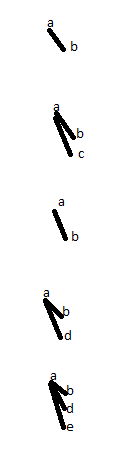
\includegraphics[height=4cm]{hw1_5_1_a.png}\\
	\end{center}
	
	And here we have the actual process tree. It looks like I was able to interpret the information correctly.
	\begin{center}
	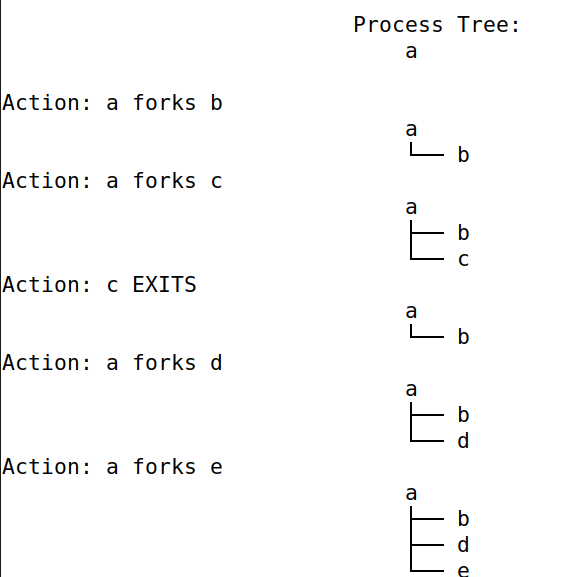
\includegraphics[width=6cm]{hw1_5_1.png}\\
	\end{center}
	. \\ \\ 

5.2

	As the percentage likelyhood for a fork increases, the number of forks on each of the processes also increases. At 0.9, every process has a fork. \\ \\ \\
	
	
5.3

	From the process tree:
	\begin{center}
	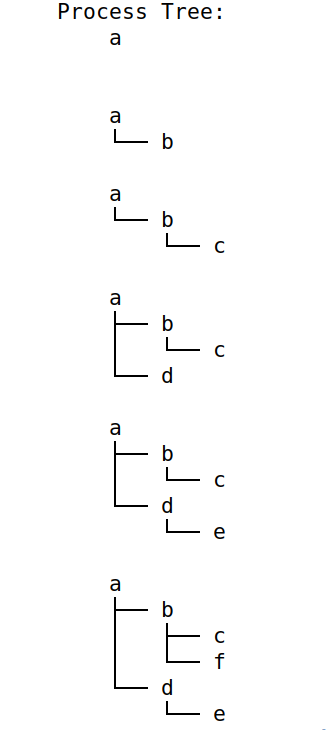
\includegraphics[height=4cm]{hw1_5_3.png}\\
	\end{center}
	it looks like the actions were:\\
	
	a forks b
	
	b forks c
	
	a forks d
	
	d forks e
	
	b forks f \\ \\ \\
	
5.4
	
	From the prompt, I assumed that when c was exited, that all the forked children of c would either dissapear of link to the parent of c, or b.  However, it looks like this only occurs on the -R flag, and otherwise the children link from a. \\ \\ \\

5.5

	From the operations, I drew the following process tree.
	
	\begin{center}
	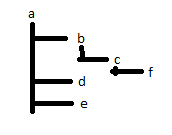
\includegraphics[height=4cm]{hw1_5_5.png}\\
	\end{center}
	
	And here is the process tree that was returned with the -c flag:
	
	\begin{center}
	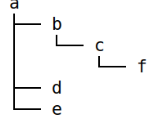
\includegraphics[height=4cm]{hw1_5_5_a.png}\\
	\end{center}
	. \\ \\ 

5.6

	Running the execution command with the relavent flags, I got:
	\begin{center}
	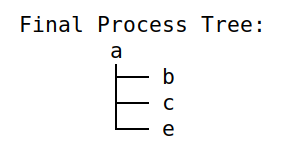
\includegraphics[height=4cm]{hw1_5_6.png}\\
	\end{center}
	To the left, there were five action tags, representing that five actions took place.
	
	I would guess that the processes were along the lines of:\\
	
	a forks b
	
	a forks c
	
	a forks d
	
	a forks e
	
	d exits
	
	Unfortunately, all I can really determine is that d was removed and the fork for e occurred after d was created. \\ \\ \\
	
	
5.1

	code in varAfterFork.c\\
	The variable does not change its value between the parent and child processes. Then, when each changes the value for x, the change does not affect the variable's value in the other process. \\ \\ \\
	
5.2

	************uncompleted**************	 \\ \\ \\
	
5.3

	code in helloGoodbye.c
	I can not guarantee that the child process will complete first, though I force the parent to wait by having it run 100000 iterations which should slow it long enough for child to finish. \\ \\ \\

5.4

	code in forkedLS.c

5.5
5.6
5.7
5.8




\end{document}  